\documentclass[aspectratio=169]{beamer}
%\documentclass{beamer}

\usetheme{LU-spfaff}
\usepackage[T1]{fontenc}
\usepackage{pgf}
\usepackage{multirow,multicol,colortbl}
\usepackage[utf8]{inputenc}
\usepackage[T1]{fontenc}

\usepackage[british]{babel}
\usepackage[scaled]{helvet}
\usepackage{tikz,pgfplots}
\usepackage{siunitx}
\pgfplotsset{compat=1.10}

\title[RIXS]{Resonant Inelastic X-Ray Scattering}

\titlecolor{LUGreen} % Choose between LUPink, LULBlue, LUIvory, LUGreen
\titleimage{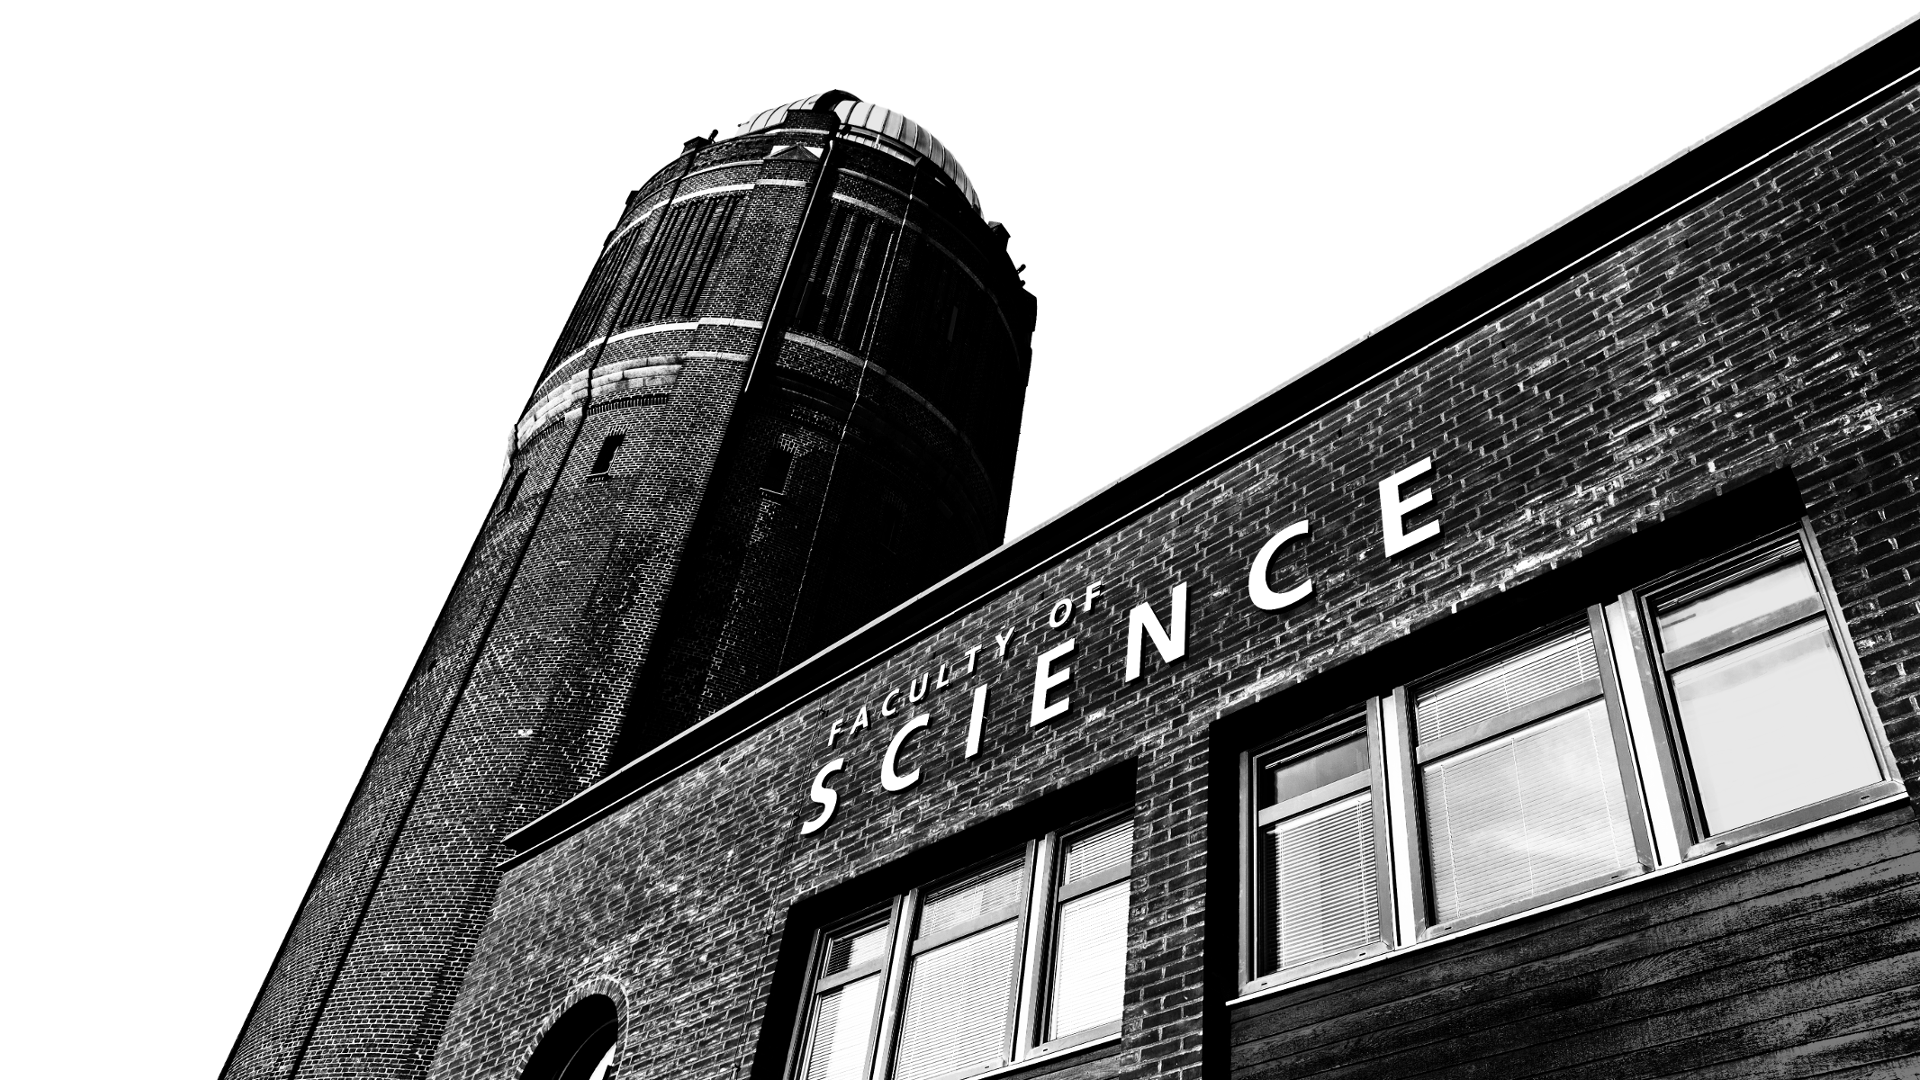
\includegraphics[scale=.5]{astro.png}}
%\titleimage{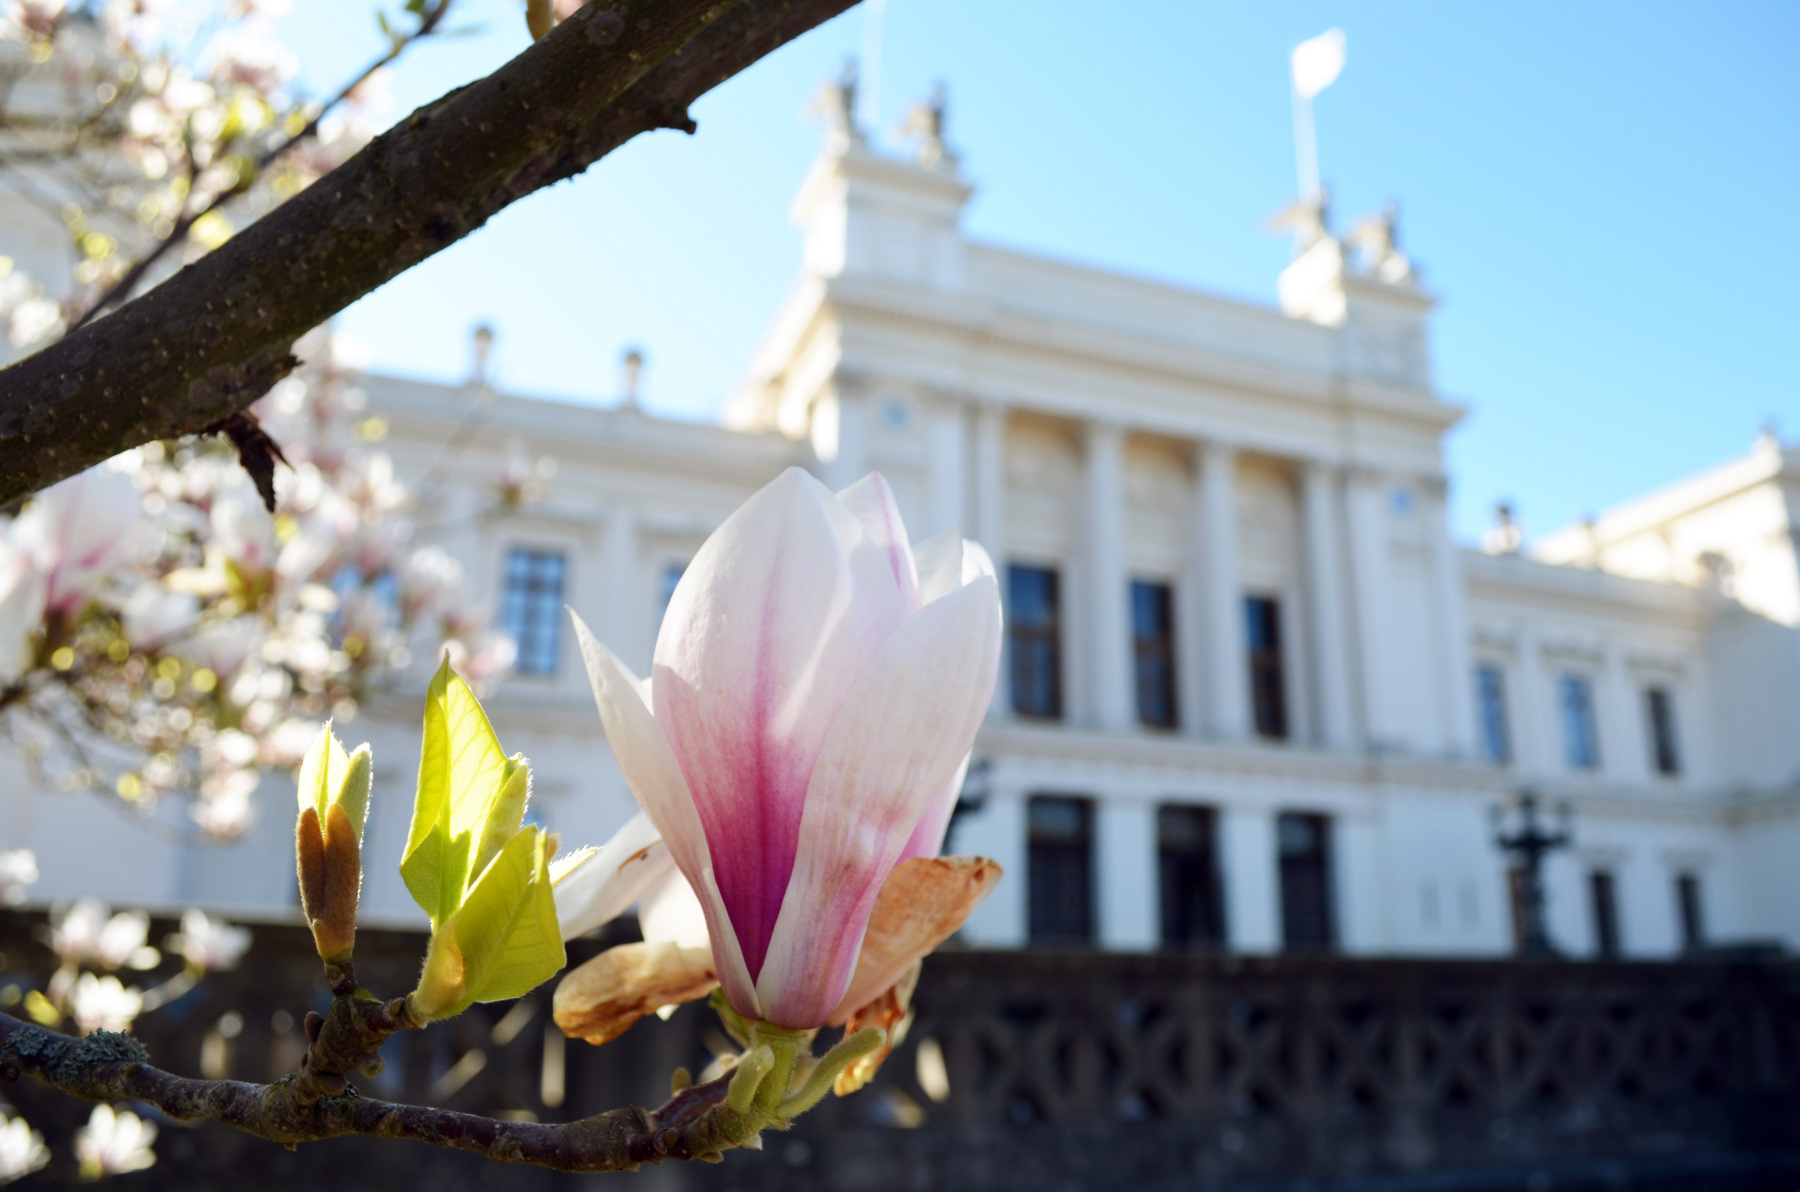
\includegraphics[scale=.6]{lumainb.jpg}}
\author{Sebastian Pfaff}
\subtitle{Another spectroscopy technique}% | More Subtitle\\Second line of subtitle}
\date{\today}
\institute{Lund University\\Department of Physics}

\begin{document}

\titleframe

\section{Motivation}
\begin{frame}{Motivation}
	\begin{columns}[onlytextwidth]
		\begin{column}{.45\textwidth}
			\includegraphics[width=\columnwidth]{nicestmpicture.jpg}
		\end{column}
		\begin{column}{.5\textwidth}
			\begin{itemize}
				\item Made possible due to advancements in synchrotron development
				\item Probe unoccupied states
				\item Gather information about dynamics
				\item Determine decay ratios
			\end{itemize}
		\end{column}
		\end{columns}
\end{frame}

\begin{frame}{Process}
	\begin{columns}[onlytextwidth]
		\begin{column}{.45\textwidth}
			\input{../paper/exscheme.tikz}
		\end{column}
		\begin{column}{.5\textwidth}
			\begin{itemize}
				\item Sample is irradiated by X-Rays at K-resonance
				\item A photon with energy $E_v-E_0$ excited an electron
				\item Various detunings may be probed to study dynamics
			\end{itemize}
		\end{column}
		\end{columns}
\end{frame}

\begin{frame}{Process}
	\begin{columns}[onlytextwidth]
		\begin{column}{.45\textwidth}
			\input{../paper/deexscheme.tikz}
		\end{column}
		\begin{column}{.5\textwidth}
			\begin{itemize}
				\item The excited electron moves back to the core electronic state
				\item This will emit a photon with energy $E_v-E_0-\delta$.
				\item Can be used to study vibrational levels
			\end{itemize}
		\end{column}
		\end{columns}
\end{frame}

\end{document}